\documentclass[10pt, letterpaper]{article}

\usepackage{tikz} 
\usepackage{pgfplots}
\pgfplotsset{compat=1.9}
\usetikzlibrary{arrows,shapes,automata,backgrounds,petri,fit,decorations.pathmorphing, calc}

\begin{document}

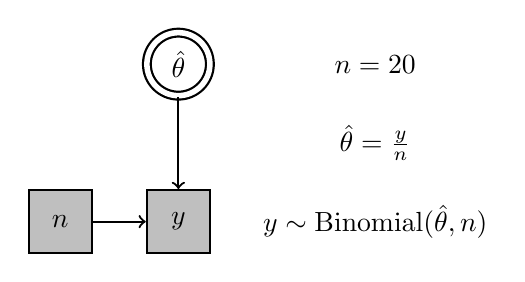
\begin{tikzpicture}[node distance = 2cm, double distance = 2pt, minimum size=.8cm, thick]
  \node[circle, draw=black, double] (theta) {$\hat \theta$};
  \node[rectangle, below of=theta, draw=black, fill=lightgray] (y) {$y$};
  \node[rectangle, draw=black, fill=lightgray, left of=y, node distance = 1.5cm] (n) {$n$};
  
  \draw[->] (theta)--(y);
  \draw[->] (n)--(y);
   
  \begin{scope}[xshift = 2.5cm, node distance = 1cm]
      \node[] at(0, 0) (n) {$n = 20$};
      \node[below of = n] (theta) {$\hat \theta = \frac{y}{n}$};
      \node[below of = theta] (y) {$y \sim \mbox{Binomial}(\hat \theta, n)$};
   \end{scope}
    
\end{tikzpicture}

\end{document}